\documentclass[12pt]{article}
\usepackage{fontspec}
\usepackage[english, russian]{babel}
\usepackage{amsmath, amssymb}
\usepackage{tikz}
\usepackage{float}

\usepackage{pgfplots}
\pgfplotsset{compat=newest}
\usetikzlibrary{arrows.meta}

\setmainfont{CMU Serif}
\setsansfont{CMU Sans Serif}
\setmonofont{CMU Typewriter Text}

\usepackage{hyperref}
\hypersetup{
    colorlinks=true,        % цветные ссылки (false - черные рамки)
    linkcolor=black,        % цвет ссылок на разделы
    urlcolor=blue,          % цвет URL-ссылок
    citecolor=green,        % цвет ссылок на литературу
    pdfborder={0 0 0}       % убрать рамки вокруг ссылок
}

\usepackage[a4paper,
            left=3cm,
            right=3cm,
            top=2cm,
            bottom=3cm]{geometry}

\begin{document}

\begin{titlepage}
    \begin{center}
        \large
        \textsc{ФГАОУ ВО «НИУ ИТМО»\\
        Факультет программной инженерии и~компьютерной~техники}
        \vspace*{4cm}
            
        \LARGE
        \textbf{Лабораторная работа №4}

        \vspace{0.5cm}
        \LARGE

        Численные методы безусловной оптимизации функции нескольких переменных
            
        \vspace{0.5cm}
        \large
        (по дисциплине «Методы оптимизации»)

        \vspace{1.5cm}

        \hfill\large
        \begin{tabular}{@{}l@{}}
        \textbf{Выполнили:}\\[2mm]
        Лабин Макар Андреевич,\\
        МОПТ 3.3, P3231, 466449;\\
        Ожеховский Александр Сергеевич,\\
        МОПТ 3.3, P3231, 466944.\\[2mm]
        \textbf{Проверил:}\\[2mm]
        Запорожцев Иван Федорович
        \end{tabular}
            
        \vfill
            
        \vspace{0.8cm}
            
        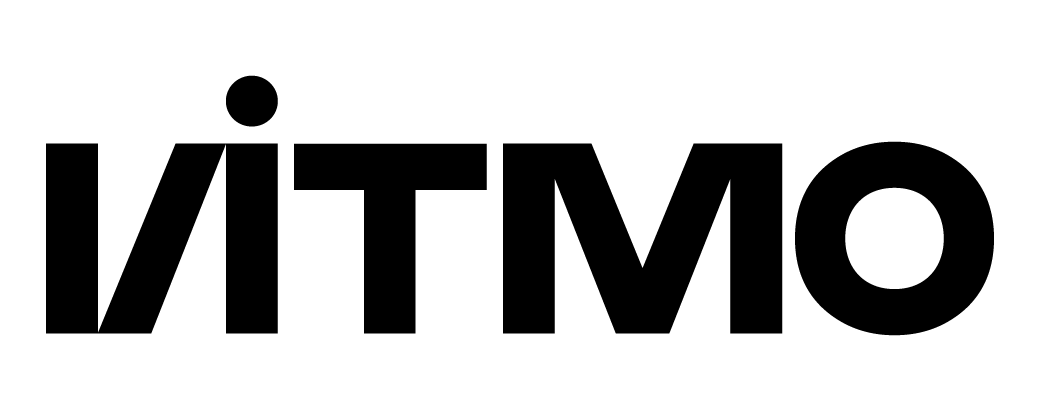
\includegraphics[width=0.4\textwidth]{itmo}
            
        \Large
        г. Санкт-Петербург, Россия\\
        2026
            
    \end{center}
\end{titlepage}

\renewcommand{\thefootnote}{[\arabic{footnote}]}

\tableofcontents
\newpage

\section{Постановка задач}

В рамках выполнения лабораторной работы \textit{по варианту №3} необходимо исследовать следующую функцию на наличие экстремумов:
\[
  f(x, y) = 1.0x^2 + 2.0y^2 + 1.0xy + -9.0x + -15.0y + 36.0
\]

Исследования необходимо производить двумя способами:
\begin{itemize}
  \item аналитически;
  \item численно:
  \begin{itemize}
    \item методом циклического покоординатного спуска;
    \item методом градиентного спуска;
    \item методом наискорейшего спуска.
  \end{itemize}
\end{itemize}

Для численных методов необходимо использовать следующие параметры:
\begin{itemize}
  \item Начальное приближение: \( x^{(0)}=(-1.0000, -2.0000)^T \).
  \item Для критерия останова: \( \varepsilon = 0.0001 \).
\end{itemize}

\newpage

\section{Аналитический метод}

Данная функция \( f(x,y) \) --- квадратичная форма. Для поиска её экстремумов воспользуемся необходимым и достаточным условиями экстремума функции нескольких переменных.

\subsection{Необходимое условие экстремума}

Найдём частные производные первого порядка и приравняем их к нулю, чтобы определить координаты стационарных точек:
\[
  \begin{cases}
    \frac{\partial f}{\partial x} = 2ax+cy+d= 2 \cdot 1.0x + 1.0y + -9.0 = 0 \\
    \frac{\partial f}{\partial y} = 2by+cx+e= 2 \cdot 2.0y + 1.0x + -15.0 = 0
  \end{cases}
\]

Решая систему, находим координаты единственной стационарной точки:
\[
x^* = 3.0000, \quad y^* = 3.0000
\]

\subsection{Достаточное условие экстремума}

Для проверки характера найденной точки составим матрицу Гессе:
\begin{equation*}
H(x, y) = \begin{pmatrix}
    \frac{\partial^2 f}{\partial x^2} & \frac{\partial^2 f}{\partial x \partial y} \\[1ex]
    \frac{\partial^2 f}{\partial y \partial x} & \frac{\partial^2 f}{\partial y^2}
\end{pmatrix}
\implies H(x^\ast, y^\ast)=
\begin{pmatrix}
    2 \cdot 1.0 & 1.0 \\
    1.0 & 2 \cdot 2.0
\end{pmatrix}
\end{equation*}

Исследуем знаки главных миноров гессиана:
\begin{itemize}
    \item \( \Delta_1 = \frac{\partial^2 f}{\partial x^2}(x^\ast,y^\ast) = 2 \cdot 1.0 = 2.0000>0 \).
    \item \( \Delta_2 = \det(H) = 4 \cdot 1.0 \cdot 2.0 - 1.0^2 = 7.0000>0 \).
\end{itemize}

По критерию Сильвестра, матрица Гессе положительно определена, то есть \( f(x,y) \) строго выпукла вниз.

Следовательно, стационарная точка есть \textit{точка глобального минимума}:
\[
x^* = (3.0000, 3.0000)^T
\]

Значение функции в точке минимума:
\[
f(x^*, y^*) = 0.0000
\]

\newpage
\section{Метод покоординатного спуска}

\subsection{Применимость метода}

Целевая функция ограничена снизу, что гарантирует сходимость метода. Задачи одномерной минимизации решаются аналитически за константное время путём поиска вершины параболы для данного направления.

\subsection{Подробный расчёт итераций}
\subsubsection{Итерация 1}

\begin{enumerate}
  \item Найдём $\alpha^{(1)}_1$ для направления $e_1=(1,0)^T$ как вершину параболы:
  \[
  \begin{gathered}
    \alpha^{(1)}_1=\textrm{arg}\,\min_{\alpha}f(x^{(0)}+\alpha e_1)=-\dfrac{2ax^{(0)}_1+cx^{(0)}_2+d}{2a}=\\
    =-\dfrac{2\cdot 1.0\cdot -1.0000+1.0\cdot -2.0000+-9.0}{2\cdot 1.0}=6.5000
  \end{gathered}
  \]

  Имеем:
  \[
    \tilde{x}_1^{(1)}=x^{(0)}+\alpha_1^{(1)}e_1=(5.5000,-2.0000)^T
  \]

  \item Аналогично найдём $\alpha^{(1)}_2$ для направления $e_2=(0,1)^T$:
  \[
  \begin{gathered}
    \alpha^{(1)}_2=\textrm{arg}\,\min_{\alpha}f(\tilde{x}^{(1)}_1+\alpha e_2)=-\dfrac{2b\tilde{x}^{(1)}_2+c\tilde{x}^{(1)}_1+e}{2b}=\\
    =-\dfrac{2\cdot 2.0\cdot -2.0000+1.0\cdot 5.5000+-15.0}{2\cdot 2.0}=4.3750
  \end{gathered}
  \]

  Итого имеем:
  \[
    x^{(1)}=\tilde{x}_2^{(1)}=\tilde{x}^{(1)}_1+\alpha_2^{(1)}e_2=(5.5000,2.3750)^T
  \]

  \item Графическая интерпретация:
  \begin{figure}[H]
  \centering
  \begin{tikzpicture}
    \begin{axis}[
      width=10cm, height=10cm,
      axis lines=middle,
      xlabel={$x$},
      ylabel={$y$},
      xlabel style={right},
      ylabel style={above},
      colormap={blackwhite}{gray(0cm)=(0.4); gray(1cm)=(0.9)},
      view={0}{90}
    ]
      \addplot3[
        contour lua={
          levels={86.0000, 43.7500, 5.4688},
          labels=false,
        },
        samples=100,
        domain=-2.0000:6.5000,
        domain y=-3.0000:3.3750,
      ] {1.0*x^2 + 2.0*y^2 + 1.0*x*y + -9.0*x + -15.0*y + 36.0};

      \addplot[, -{Stealth[scale=0.8]}] coordinates {(-1.000, -2.000) (5.500, -2.000)};
\addplot[, -{Stealth[scale=0.8]}] coordinates {(5.500, -2.000) (5.500, 2.375)};
\addplot[fill=black, mark=*, mark size=1pt] coordinates {(-1.000, -2.000)};
\addplot[fill=black, mark=*, mark size=1pt] coordinates {(5.500, -2.000)};
\addplot[fill=black, mark=*, mark size=1pt] coordinates {(5.500, 2.375)};
        
    \end{axis}
  \end{tikzpicture}
  \caption{Итерация №1 метода циклического покоординатного спуска.}
  \end{figure}

  \item Проверка критерия останова:
  \[
    |x^{(1)}-x^{(0)}|=7.8352\geq 0.0001\implies\text{продолжаем алгоритм.}
  \]
\end{enumerate}\subsubsection{Итерация 2}

\begin{enumerate}
  \item Найдём $\alpha^{(2)}_1$ для направления $e_1=(1,0)^T$ как вершину параболы:
  \[
  \begin{gathered}
    \alpha^{(2)}_1=\textrm{arg}\,\min_{\alpha}f(x^{(1)}+\alpha e_1)=-\dfrac{2ax^{(1)}_1+cx^{(1)}_2+d}{2a}=\\
    =-\dfrac{2\cdot 1.0\cdot 5.5000+1.0\cdot 2.3750+-9.0}{2\cdot 1.0}=-2.1875
  \end{gathered}
  \]

  Имеем:
  \[
    \tilde{x}_1^{(1)}=x^{(0)}+\alpha_1^{(1)}e_1=(3.3125,2.3750)^T
  \]

  \item Аналогично найдём $\alpha^{(2)}_2$ для направления $e_2=(0,1)^T$:
  \[
  \begin{gathered}
    \alpha^{(2)}_2=\textrm{arg}\,\min_{\alpha}f(\tilde{x}^{(1)}_1+\alpha e_2)=-\dfrac{2b\tilde{x}^{(2)}_2+c\tilde{x}^{(2)}_1+e}{2b}=\\
    =-\dfrac{2\cdot 2.0\cdot 2.3750+1.0\cdot 3.3125+-15.0}{2\cdot 2.0}=0.5469
  \end{gathered}
  \]

  Итого имеем:
  \[
    x^{(1)}=\tilde{x}_2^{(1)}=\tilde{x}^{(1)}_1+\alpha_2^{(1)}e_2=(3.3125,2.9219)^T
  \]

  \item Графическая интерпретация:
  \begin{figure}[H]
  \centering
  \begin{tikzpicture}
    \begin{axis}[
      width=10cm, height=10cm,
      axis lines=middle,
      xlabel={$x$},
      ylabel={$y$},
      xlabel style={right},
      ylabel style={above},
      colormap={blackwhite}{gray(0cm)=(0.4); gray(1cm)=(0.9)},
      view={0}{90}
    ]
      \addplot3[
        contour lua={
          levels={86.0000, 43.7500, 5.4688, 0.6836, 0.0854},
          labels=false,
        },
        samples=100,
        domain=-2.0000:6.5000,
        domain y=-3.0000:3.9219,
      ] {1.0*x^2 + 2.0*y^2 + 1.0*x*y + -9.0*x + -15.0*y + 36.0};

      \addplot[thin, gray!80, dashed, -{Stealth[scale=0.8]}] coordinates {(-1.000, -2.000) (5.500, -2.000)};
\addplot[thin, gray!80, dashed, -{Stealth[scale=0.8]}] coordinates {(5.500, -2.000) (5.500, 2.375)};
\addplot[mark=*, mark size=1pt, draw=gray, fill=gray] coordinates {(-1.000, -2.000)};
\addplot[mark=*, mark size=1pt, draw=gray, fill=gray] coordinates {(5.500, -2.000)};
\addplot[, -{Stealth[scale=0.8]}] coordinates {(5.500, 2.375) (3.312, 2.375)};
\addplot[, -{Stealth[scale=0.8]}] coordinates {(3.312, 2.375) (3.312, 2.922)};
\addplot[fill=black, mark=*, mark size=1pt] coordinates {(5.500, 2.375)};
\addplot[fill=black, mark=*, mark size=1pt] coordinates {(3.312, 2.375)};
\addplot[fill=black, mark=*, mark size=1pt] coordinates {(3.312, 2.922)};
        
    \end{axis}
  \end{tikzpicture}
  \caption{Итерация №2 метода циклического покоординатного спуска.}
  \end{figure}

  \item Проверка критерия останова:
  \[
    |x^{(2)}-x^{(1)}|=2.2548\geq 0.0001\implies\text{продолжаем алгоритм.}
  \]
\end{enumerate}\subsubsection{Итерация 3}

\begin{enumerate}
  \item Найдём $\alpha^{(3)}_1$ для направления $e_1=(1,0)^T$ как вершину параболы:
  \[
  \begin{gathered}
    \alpha^{(3)}_1=\textrm{arg}\,\min_{\alpha}f(x^{(2)}+\alpha e_1)=-\dfrac{2ax^{(2)}_1+cx^{(2)}_2+d}{2a}=\\
    =-\dfrac{2\cdot 1.0\cdot 3.3125+1.0\cdot 2.9219+-9.0}{2\cdot 1.0}=-0.2734
  \end{gathered}
  \]

  Имеем:
  \[
    \tilde{x}_1^{(1)}=x^{(0)}+\alpha_1^{(1)}e_1=(3.0391,2.9219)^T
  \]

  \item Аналогично найдём $\alpha^{(3)}_2$ для направления $e_2=(0,1)^T$:
  \[
  \begin{gathered}
    \alpha^{(3)}_2=\textrm{arg}\,\min_{\alpha}f(\tilde{x}^{(1)}_1+\alpha e_2)=-\dfrac{2b\tilde{x}^{(3)}_2+c\tilde{x}^{(3)}_1+e}{2b}=\\
    =-\dfrac{2\cdot 2.0\cdot 2.9219+1.0\cdot 3.0391+-15.0}{2\cdot 2.0}=0.0684
  \end{gathered}
  \]

  Итого имеем:
  \[
    x^{(1)}=\tilde{x}_2^{(1)}=\tilde{x}^{(1)}_1+\alpha_2^{(1)}e_2=(3.0391,2.9902)^T
  \]

  \item Графическая интерпретация:
  \begin{figure}[H]
  \centering
  \begin{tikzpicture}
    \begin{axis}[
      width=10cm, height=10cm,
      axis lines=middle,
      xlabel={$x$},
      ylabel={$y$},
      xlabel style={right},
      ylabel style={above},
      colormap={blackwhite}{gray(0cm)=(0.4); gray(1cm)=(0.9)},
      view={0}{90}
    ]
      \addplot3[
        contour lua={
          levels={86.0000, 43.7500, 5.4688, 0.6836, 0.0854, 0.0107, 0.0013},
          labels=false,
        },
        samples=100,
        domain=-2.0000:6.5000,
        domain y=-3.0000:3.9902,
      ] {1.0*x^2 + 2.0*y^2 + 1.0*x*y + -9.0*x + -15.0*y + 36.0};

      \addplot[thin, gray!80, dashed, -{Stealth[scale=0.8]}] coordinates {(-1.000, -2.000) (5.500, -2.000)};
\addplot[thin, gray!80, dashed, -{Stealth[scale=0.8]}] coordinates {(5.500, -2.000) (5.500, 2.375)};
\addplot[mark=*, mark size=1pt, draw=gray, fill=gray] coordinates {(-1.000, -2.000)};
\addplot[mark=*, mark size=1pt, draw=gray, fill=gray] coordinates {(5.500, -2.000)};
\addplot[thin, gray!80, dashed, -{Stealth[scale=0.8]}] coordinates {(5.500, 2.375) (3.312, 2.375)};
\addplot[thin, gray!80, dashed, -{Stealth[scale=0.8]}] coordinates {(3.312, 2.375) (3.312, 2.922)};
\addplot[mark=*, mark size=1pt, draw=gray, fill=gray] coordinates {(5.500, 2.375)};
\addplot[mark=*, mark size=1pt, draw=gray, fill=gray] coordinates {(3.312, 2.375)};
\addplot[, -{Stealth[scale=0.8]}] coordinates {(3.312, 2.922) (3.039, 2.922)};
\addplot[, -{Stealth[scale=0.8]}] coordinates {(3.039, 2.922) (3.039, 2.990)};
\addplot[fill=black, mark=*, mark size=1pt] coordinates {(3.312, 2.922)};
\addplot[fill=black, mark=*, mark size=1pt] coordinates {(3.039, 2.922)};
\addplot[fill=black, mark=*, mark size=1pt] coordinates {(3.039, 2.990)};
        
    \end{axis}
  \end{tikzpicture}
  \caption{Итерация №3 метода циклического покоординатного спуска.}
  \end{figure}

  \item Проверка критерия останова:
  \[
    |x^{(3)}-x^{(2)}|=0.2819\geq 0.0001\implies\text{продолжаем алгоритм.}
  \]
\end{enumerate}

\subsection{Сводная таблица итераций}
\begin{table}[H]
\centering
\begin{tabular}{|c|c|c|c|c|}
\hline
$k$ & $x^{(k-1)}$ & $\alpha^{(k)}$ & $x^{(k)}$ & $|x^{(k)} - x^{(k-1)}|$ \\
\hline
1 & $(-1.0000, -2.0000)^T$ & $(6.5000, 4.3750)^T$ & $(5.5000, 2.3750)^T$ & $7.8352$ \\
\hline
2 & $(5.5000, 2.3750)^T$ & $(-2.1875, 0.5469)^T$ & $(3.3125, 2.9219)^T$ & $2.2548$ \\
\hline
3 & $(3.3125, 2.9219)^T$ & $(-0.2734, 0.0684)^T$ & $(3.0391, 2.9902)^T$ & $0.2819$ \\
\hline
4 & $(3.0391, 2.9902)^T$ & $(-0.0342, 0.0085)^T$ & $(3.0049, 2.9988)^T$ & $0.0352$ \\
\hline
5 & $(3.0049, 2.9988)^T$ & $(-0.0043, 0.0011)^T$ & $(3.0006, 2.9998)^T$ & $0.0044$ \\
\hline
6 & $(3.0006, 2.9998)^T$ & $(-0.0005, 0.0001)^T$ & $(3.0001, 3.0000)^T$ & $0.0006$ \\
\hline
7 & $(3.0001, 3.0000)^T$ & $(-0.0001, 0.0000)^T$ & $(3.0000, 3.0000)^T$ & $0.0001$ \\
\hline

\end{tabular}
\end{table}

Итого имеем:
\[
  \tilde{x}^{\ast}=(3.0000, 3.0000)^T
\]

\subsection{График спусков}

\begin{figure}[H]
  \centering
  \begin{tikzpicture}
    \begin{axis}[
      width=10cm, height=10cm,
      axis lines=middle,
      xlabel={$x$},
      ylabel={$y$},
      xlabel style={right},
      ylabel style={above},
      colormap={blackwhite}{gray(0cm)=(0.4); gray(1cm)=(0.9)},
      view={0}{90}
    ]
      \addplot3[
        contour lua={
          number=10,
          labels=false,
        },
        samples=30,
        domain=-2.0:6.5,
        domain y=-3.0:3.999997615814209,
      ] {1.0*x^2 + 2.0*y^2 + 1.0*x*y + -9.0*x + -15.0*y + 36.0};

      \addplot[thin, gray!80, dashed, -{Stealth[scale=0.8]}] coordinates {(-1.000, -2.000) (5.500, -2.000)};
\addplot[thin, gray!80, dashed, -{Stealth[scale=0.8]}] coordinates {(5.500, -2.000) (5.500, 2.375)};
\addplot[mark=*, mark size=1pt, draw=gray, fill=gray] coordinates {(-1.000, -2.000)};
\addplot[mark=*, mark size=1pt, draw=gray, fill=gray] coordinates {(5.500, -2.000)};
\addplot[thin, gray!80, dashed, -{Stealth[scale=0.8]}] coordinates {(5.500, 2.375) (3.312, 2.375)};
\addplot[thin, gray!80, dashed, -{Stealth[scale=0.8]}] coordinates {(3.312, 2.375) (3.312, 2.922)};
\addplot[mark=*, mark size=1pt, draw=gray, fill=gray] coordinates {(5.500, 2.375)};
\addplot[mark=*, mark size=1pt, draw=gray, fill=gray] coordinates {(3.312, 2.375)};
\addplot[thin, gray!80, dashed, -{Stealth[scale=0.8]}] coordinates {(3.312, 2.922) (3.039, 2.922)};
\addplot[thin, gray!80, dashed, -{Stealth[scale=0.8]}] coordinates {(3.039, 2.922) (3.039, 2.990)};
\addplot[mark=*, mark size=1pt, draw=gray, fill=gray] coordinates {(3.312, 2.922)};
\addplot[mark=*, mark size=1pt, draw=gray, fill=gray] coordinates {(3.039, 2.922)};
\addplot[thin, gray!80, dashed, -{Stealth[scale=0.8]}] coordinates {(3.039, 2.990) (3.005, 2.990)};
\addplot[thin, gray!80, dashed, -{Stealth[scale=0.8]}] coordinates {(3.005, 2.990) (3.005, 2.999)};
\addplot[mark=*, mark size=1pt, draw=gray, fill=gray] coordinates {(3.039, 2.990)};
\addplot[mark=*, mark size=1pt, draw=gray, fill=gray] coordinates {(3.005, 2.990)};
\addplot[thin, gray!80, dashed, -{Stealth[scale=0.8]}] coordinates {(3.005, 2.999) (3.001, 2.999)};
\addplot[thin, gray!80, dashed, -{Stealth[scale=0.8]}] coordinates {(3.001, 2.999) (3.001, 3.000)};
\addplot[mark=*, mark size=1pt, draw=gray, fill=gray] coordinates {(3.005, 2.999)};
\addplot[mark=*, mark size=1pt, draw=gray, fill=gray] coordinates {(3.001, 2.999)};
\addplot[thin, gray!80, dashed, -{Stealth[scale=0.8]}] coordinates {(3.001, 3.000) (3.000, 3.000)};
\addplot[thin, gray!80, dashed, -{Stealth[scale=0.8]}] coordinates {(3.000, 3.000) (3.000, 3.000)};
\addplot[mark=*, mark size=1pt, draw=gray, fill=gray] coordinates {(3.001, 3.000)};
\addplot[mark=*, mark size=1pt, draw=gray, fill=gray] coordinates {(3.000, 3.000)};
\addplot[, -{Stealth[scale=0.8]}] coordinates {(3.000, 3.000) (3.000, 3.000)};
\addplot[, -{Stealth[scale=0.8]}] coordinates {(3.000, 3.000) (3.000, 3.000)};
\addplot[fill=black, mark=*, mark size=1pt] coordinates {(3.000, 3.000)};
\addplot[fill=black, mark=*, mark size=1pt] coordinates {(3.000, 3.000)};
\addplot[fill=black, mark=*, mark size=1pt] coordinates {(3.000, 3.000)};
        
    \end{axis}
  \end{tikzpicture}
  \caption{Все итерации метода циклического покоординатного спуска.}
\end{figure}

\newpage

\section{Метод градиентного спуска}

\subsection{Применимость метода}

Целевая функция ограничена снизу, что гарантирует сходимость метода. Также она непрерывно дифференцируема на \( \mathbb{R}^2 \), что позволяет считать антиградиенты в любой точке плоскости.

Установим скорость обучения постоянной:
\[
  \eta = 0.225
\]

\subsection{Подробный расчёт итераций}
\subsubsection{Итерация 1}

\begin{enumerate}
  \item Найдём значение градиента $\omega^{(1)}=\textrm{grad}\,f(x^{(0)})$:
  \[
  \begin{gathered}
    \omega^{(1)}=(2ax_1^{(0)}+cx_2^{(0)}+d,2bx_2^{(0)}+cx_1^{(0)}+e)^T=\\
    =(2\cdot 1.0\cdot -1.0000+1.0\cdot -2.0000+-9.0, 2\cdot 2.0\cdot -2.0000+1.0\cdot -1.0000+-15.0)^T=\\
    =(-13.0000, -24.0000)^T
  \end{gathered}
  \]

  \item Вычислим \( x^{(1)} \):
  \[
    x^{(1)}=x^{(0)}-\eta\omega^{(1)}=(1.9250,3.4000)^T
  \]

  \item Графическая интерпретация:
  \begin{figure}[H]
  \centering
  \begin{tikzpicture}
    \begin{axis}[
      width=10cm, height=10cm,
      axis lines=middle,
      xlabel={$x$},
      ylabel={$y$},
      xlabel style={right},
      ylabel style={above},
      colormap={blackwhite}{gray(0cm)=(0.4); gray(1cm)=(0.9)},
      view={0}{90}
    ]
      \addplot3[
        contour lua={
          levels={86.0000, 1.0456},
          labels=false,
        },
        samples=100,
        domain=-2.0000:2.9250,
        domain y=-3.0000:4.4000,
      ] {1.0*x^2 + 2.0*y^2 + 1.0*x*y + -9.0*x + -15.0*y + 36.0};

      \addplot[, -Stealth] coordinates {(-1.000, -2.000) (1.925, 3.400)};
\addplot[fill=black, mark=*, mark size=1pt] coordinates {(1.925, 3.400)};
        
    \end{axis}
  \end{tikzpicture}
  \caption{Итерация №1 метода градиентного спуска.}
  \end{figure}

  \item Проверка критерия останова:
  \[
    |\omega^{(1)}|=27.2947\geq 0.0001\implies\text{продолжаем алгоритм.}
  \]
\end{enumerate}
\subsubsection{Итерация 2}

\begin{enumerate}
  \item Найдём значение градиента $\omega^{(2)}=\textrm{grad}\,f(x^{(1)})$:
  \[
  \begin{gathered}
    \omega^{(2)}=(2ax_1^{(1)}+cx_2^{(1)}+d,2bx_2^{(1)}+cx_1^{(1)}+e)^T=\\
    =(2\cdot 1.0\cdot 1.9250+1.0\cdot 3.4000+-9.0, 2\cdot 2.0\cdot 3.4000+1.0\cdot 1.9250+-15.0)^T=\\
    =(-1.7500, 0.5250)^T
  \end{gathered}
  \]

  \item Вычислим \( x^{(2)} \):
  \[
    x^{(2)}=x^{(1)}-\eta\omega^{(2)}=(2.3188,3.2819)^T
  \]

  \item Графическая интерпретация:
  \begin{figure}[H]
  \centering
  \begin{tikzpicture}
    \begin{axis}[
      width=10cm, height=10cm,
      axis lines=middle,
      xlabel={$x$},
      ylabel={$y$},
      xlabel style={right},
      ylabel style={above},
      colormap={blackwhite}{gray(0cm)=(0.4); gray(1cm)=(0.9)},
      view={0}{90}
    ]
      \addplot3[
        contour lua={
          levels={86.0000, 1.0456, 0.4310},
          labels=false,
        },
        samples=100,
        domain=-2.0000:3.3188,
        domain y=-3.0000:4.4000,
      ] {1.0*x^2 + 2.0*y^2 + 1.0*x*y + -9.0*x + -15.0*y + 36.0};

      \addplot[thin, gray!80, dashed, -Stealth] coordinates {(-1.000, -2.000) (1.925, 3.400)};
\addplot[, -Stealth] coordinates {(1.925, 3.400) (2.319, 3.282)};
\addplot[fill=black, mark=*, mark size=1pt] coordinates {(2.319, 3.282)};
        
    \end{axis}
  \end{tikzpicture}
  \caption{Итерация №2 метода градиентного спуска.}
  \end{figure}

  \item Проверка критерия останова:
  \[
    |\omega^{(2)}|=1.8271\geq 0.0001\implies\text{продолжаем алгоритм.}
  \]
\end{enumerate}
\subsubsection{Итерация 3}

\begin{enumerate}
  \item Найдём значение градиента $\omega^{(3)}=\textrm{grad}\,f(x^{(2)})$:
  \[
  \begin{gathered}
    \omega^{(3)}=(2ax_1^{(2)}+cx_2^{(2)}+d,2bx_2^{(2)}+cx_1^{(2)}+e)^T=\\
    =(2\cdot 1.0\cdot 2.3188+1.0\cdot 3.2819+-9.0, 2\cdot 2.0\cdot 3.2819+1.0\cdot 2.3188+-15.0)^T=\\
    =(-1.0806, 0.4462)^T
  \end{gathered}
  \]

  \item Вычислим \( x^{(3)} \):
  \[
    x^{(3)}=x^{(2)}-\eta\omega^{(3)}=(2.5619,3.1815)^T
  \]

  \item Графическая интерпретация:
  \begin{figure}[H]
  \centering
  \begin{tikzpicture}
    \begin{axis}[
      width=10cm, height=10cm,
      axis lines=middle,
      xlabel={$x$},
      ylabel={$y$},
      xlabel style={right},
      ylabel style={above},
      colormap={blackwhite}{gray(0cm)=(0.4); gray(1cm)=(0.9)},
      view={0}{90}
    ]
      \addplot3[
        contour lua={
          levels={86.0000, 1.0456, 0.4310, 0.1783},
          labels=false,
        },
        samples=100,
        domain=-2.0000:3.5619,
        domain y=-3.0000:4.4000,
      ] {1.0*x^2 + 2.0*y^2 + 1.0*x*y + -9.0*x + -15.0*y + 36.0};

      \addplot[thin, gray!80, dashed, -Stealth] coordinates {(-1.000, -2.000) (1.925, 3.400)};
\addplot[thin, gray!80, dashed, -Stealth] coordinates {(1.925, 3.400) (2.319, 3.282)};
\addplot[, -Stealth] coordinates {(2.319, 3.282) (2.562, 3.181)};
\addplot[fill=black, mark=*, mark size=1pt] coordinates {(2.562, 3.181)};
        
    \end{axis}
  \end{tikzpicture}
  \caption{Итерация №3 метода градиентного спуска.}
  \end{figure}

  \item Проверка критерия останова:
  \[
    |\omega^{(3)}|=1.1691\geq 0.0001\implies\text{продолжаем алгоритм.}
  \]
\end{enumerate}


\subsection{Сводная таблица итераций}
\begin{table}[H]
\centering
\begin{tabular}{|c|c|c|c|c|}
\hline
$k$ & $x^{(k-1)}$ & $\omega^{(k)}$ & $x^{(k)}$ & $|\omega^{(k)}|$ \\
\hline
1 & $(-1.0000, -2.0000)^T$ & $(-13.0000, -24.0000)^T$ & $(1.9250, 3.4000)^T$ & $27.2947$ \\
\hline
2 & $(1.9250, 3.4000)^T$ & $(-1.7500, 0.5250)^T$ & $(2.3188, 3.2819)^T$ & $1.8271$ \\
\hline
3 & $(2.3188, 3.2819)^T$ & $(-1.0806, 0.4462)^T$ & $(2.5619, 3.1815)^T$ & $1.1691$ \\
\hline
4 & $(2.5619, 3.1815)^T$ & $(-0.6947, 0.2878)^T$ & $(2.7182, 3.1167)^T$ & $0.7520$ \\
\hline
5 & $(2.7182, 3.1167)^T$ & $(-0.4469, 0.1851)^T$ & $(2.8188, 3.0751)^T$ & $0.4837$ \\
\hline
6 & $(2.8188, 3.0751)^T$ & $(-0.2874, 0.1191)^T$ & $(2.8834, 3.0483)^T$ & $0.3111$ \\
\hline
7 & $(2.8834, 3.0483)^T$ & $(-0.1849, 0.0766)^T$ & $(2.9250, 3.0311)^T$ & $0.2001$ \\
\hline
8 & $(2.9250, 3.0311)^T$ & $(-0.1189, 0.0493)^T$ & $(2.9518, 3.0200)^T$ & $0.1287$ \\
\hline
9 & $(2.9518, 3.0200)^T$ & $(-0.0765, 0.0317)^T$ & $(2.9690, 3.0128)^T$ & $0.0828$ \\
\hline
10 & $(2.9690, 3.0128)^T$ & $(-0.0492, 0.0204)^T$ & $(2.9800, 3.0083)^T$ & $0.0532$ \\
\hline
11 & $(2.9800, 3.0083)^T$ & $(-0.0316, 0.0131)^T$ & $(2.9872, 3.0053)^T$ & $0.0342$ \\
\hline
12 & $(2.9872, 3.0053)^T$ & $(-0.0204, 0.0084)^T$ & $(2.9917, 3.0034)^T$ & $0.0220$ \\
\hline
13 & $(2.9917, 3.0034)^T$ & $(-0.0131, 0.0054)^T$ & $(2.9947, 3.0022)^T$ & $0.0142$ \\
\hline
14 & $(2.9947, 3.0022)^T$ & $(-0.0084, 0.0035)^T$ & $(2.9966, 3.0014)^T$ & $0.0091$ \\
\hline
15 & $(2.9966, 3.0014)^T$ & $(-0.0054, 0.0022)^T$ & $(2.9978, 3.0009)^T$ & $0.0059$ \\
\hline
16 & $(2.9978, 3.0009)^T$ & $(-0.0035, 0.0014)^T$ & $(2.9986, 3.0006)^T$ & $0.0038$ \\
\hline
17 & $(2.9986, 3.0006)^T$ & $(-0.0022, 0.0009)^T$ & $(2.9991, 3.0004)^T$ & $0.0024$ \\
\hline
18 & $(2.9991, 3.0004)^T$ & $(-0.0014, 0.0006)^T$ & $(2.9994, 3.0002)^T$ & $0.0016$ \\
\hline
19 & $(2.9994, 3.0002)^T$ & $(-0.0009, 0.0004)^T$ & $(2.9996, 3.0002)^T$ & $0.0010$ \\
\hline
20 & $(2.9996, 3.0002)^T$ & $(-0.0006, 0.0002)^T$ & $(2.9998, 3.0001)^T$ & $0.0006$ \\
\hline
21 & $(2.9998, 3.0001)^T$ & $(-0.0004, 0.0002)^T$ & $(2.9998, 3.0001)^T$ & $0.0004$ \\
\hline
22 & $(2.9998, 3.0001)^T$ & $(-0.0002, 0.0001)^T$ & $(2.9999, 3.0000)^T$ & $0.0003$ \\
\hline
23 & $(2.9999, 3.0000)^T$ & $(-0.0002, 0.0001)^T$ & $(2.9999, 3.0000)^T$ & $0.0002$ \\
\hline
24 & $(2.9999, 3.0000)^T$ & $(-0.0001, 0.0000)^T$ & $(3.0000, 3.0000)^T$ & $0.0001$ \\
\hline
25 & $(3.0000, 3.0000)^T$ & $(-0.0001, 0.0000)^T$ & $(3.0000, 3.0000)^T$ & $0.0001$ \\
\hline

\end{tabular}
\end{table}

Итого имеем:
\[
  \tilde{x}^{\ast}=(3.0000, 3.0000)^T
\]

\subsection{График спусков}

\begin{figure}[H]
  \centering
  \begin{tikzpicture}
    \begin{axis}[
      width=10cm, height=10cm,
      axis lines=middle,
      xlabel={$x$},
      ylabel={$y$},
      xlabel style={right},
      ylabel style={above},
      colormap={blackwhite}{gray(0cm)=(0.4); gray(1cm)=(0.9)},
      view={0}{90}
    ]
      \addplot3[
        contour lua={
          number=10,
          labels=false,
        },
        samples=30,
        domain=-2.0:3.999973382598537,
        domain y=-3.0:4.4,
      ] {1.0*x^2 + 2.0*y^2 + 1.0*x*y + -9.0*x + -15.0*y + 36.0};

      \addplot[thin, gray!80, dashed, -Stealth] coordinates {(-1.000, -2.000) (1.925, 3.400)};
\addplot[thin, gray!80, dashed, -Stealth] coordinates {(1.925, 3.400) (2.319, 3.282)};
\addplot[thin, gray!80, dashed, -Stealth] coordinates {(2.319, 3.282) (2.562, 3.181)};
\addplot[thin, gray!80, dashed, -Stealth] coordinates {(2.562, 3.181) (2.718, 3.117)};
\addplot[thin, gray!80, dashed, -Stealth] coordinates {(2.718, 3.117) (2.819, 3.075)};
\addplot[thin, gray!80, dashed, -Stealth] coordinates {(2.819, 3.075) (2.883, 3.048)};
\addplot[thin, gray!80, dashed, -Stealth] coordinates {(2.883, 3.048) (2.925, 3.031)};
\addplot[thin, gray!80, dashed, -Stealth] coordinates {(2.925, 3.031) (2.952, 3.020)};
\addplot[thin, gray!80, dashed, -Stealth] coordinates {(2.952, 3.020) (2.969, 3.013)};
\addplot[thin, gray!80, dashed, -Stealth] coordinates {(2.969, 3.013) (2.980, 3.008)};
\addplot[thin, gray!80, dashed, -Stealth] coordinates {(2.980, 3.008) (2.987, 3.005)};
\addplot[thin, gray!80, dashed, -Stealth] coordinates {(2.987, 3.005) (2.992, 3.003)};
\addplot[thin, gray!80, dashed, -Stealth] coordinates {(2.992, 3.003) (2.995, 3.002)};
\addplot[thin, gray!80, dashed, -Stealth] coordinates {(2.995, 3.002) (2.997, 3.001)};
\addplot[thin, gray!80, dashed, -Stealth] coordinates {(2.997, 3.001) (2.998, 3.001)};
\addplot[thin, gray!80, dashed, -Stealth] coordinates {(2.998, 3.001) (2.999, 3.001)};
\addplot[thin, gray!80, dashed, -Stealth] coordinates {(2.999, 3.001) (2.999, 3.000)};
\addplot[thin, gray!80, dashed, -Stealth] coordinates {(2.999, 3.000) (2.999, 3.000)};
\addplot[thin, gray!80, dashed, -Stealth] coordinates {(2.999, 3.000) (3.000, 3.000)};
\addplot[thin, gray!80, dashed, -Stealth] coordinates {(3.000, 3.000) (3.000, 3.000)};
\addplot[thin, gray!80, dashed, -Stealth] coordinates {(3.000, 3.000) (3.000, 3.000)};
\addplot[thin, gray!80, dashed, -Stealth] coordinates {(3.000, 3.000) (3.000, 3.000)};
\addplot[thin, gray!80, dashed, -Stealth] coordinates {(3.000, 3.000) (3.000, 3.000)};
\addplot[thin, gray!80, dashed, -Stealth] coordinates {(3.000, 3.000) (3.000, 3.000)};
\addplot[, -Stealth] coordinates {(3.000, 3.000) (3.000, 3.000)};
\addplot[fill=black, mark=*, mark size=1pt] coordinates {(3.000, 3.000)};
        
    \end{axis}
  \end{tikzpicture}
  \caption{Все итерации метода градиентного спуска.}
  \end{figure}

\newpage

\section{Метод наискорейшего спуска}

\subsection{Применимость метода}

Целевая функция ограничена снизу, что гарантирует сходимость метода. Также она непрерывно дифференцируема на \( \mathbb{R}^2 \), что позволяет считать антиградиенты в любой точке плоскости. Задачи одномерной минимизации решаются аналитически за константное время путём поиска вершины параболы для данного направления.

\subsection{Подробный расчёт итераций}
\subsubsection{Итерация 1}

\begin{enumerate}
  \item Найдём значение градиента $\omega^{(1)}=\textrm{grad}\,f(x^{(0)})$:
  \[
  \begin{gathered}
    \omega^{(1)}=(2ax_1^{(0)}+cx_2^{(0)}+d,2bx_2^{(0)}+cx_1^{(0)}+e)^T=\\
    =(2\cdot 1.0\cdot -1.0000+1.0\cdot -2.0000+-9.0, 2\cdot 2.0\cdot -2.0000+1.0\cdot -1.0000+-15.0)^T=(-13.0000, -24.0000)^T
  \end{gathered}
  \]

  \item Нормируем антиградиент \( \omega^{(1)} \), чтобы получить орт:
  \[
    u^{(1)}=-\dfrac{\omega^{(1)}}{|\omega^{(1)}|}=-\dfrac{(-13.0000, -24.0000)^T}{27.2947}=(0.4763,0.8793)
  \]

  \item Найдём \( \beta^{(1)} \) как вершину параболы:
  \[
  \begin{gathered}
    \beta^{(1)}_1=\textrm{arg}\,\min_{\beta}f(x^{(0)}+\beta u^{(1)})=\\
    =-\dfrac{2ax^{(0)}_1u_1^{(1)}+2bx_2^{(0)}u_2^{(1)}+c(x_1^{(1)}u_2^{(1)}+x^{(0)}_2u_1^{(1)})+du_1^{(1)}+eu_2^{(1)}}{2(a(u_1^{(1)})^2)+b(u_2^{(1)})^2+cu_1^{(1)}u_2^{(1)}}=\\
    =-\dfrac{2\cdot 1.0\cdot -1.0000\cdot 0.4763+\dots+-9.0\cdot 0.4763+-15.0\cdot 0.8793}{2\cdot (1.0\cdot(0.4763)^2+2.0\cdot (0.8793)^2+1.0\cdot 0.4763\cdot 0.8793)}=6.2261
  \end{gathered}
  \]

  \item Вычислим \( x^{(1)} \):
  \[
    x^{(1)}=x^{(0)}+\beta^{(1)}\cdot u^{(1)}=(1.9654,3.4746)^T
  \]

  \item Графическая интерпретация:
  \begin{figure}[H]
  \centering
  \begin{tikzpicture}
    \begin{axis}[
      width=10cm, height=10cm,
      axis lines=middle,
      xlabel={$x$},
      ylabel={$y$},
      xlabel style={right},
      ylabel style={above},
      colormap={blackwhite}{gray(0cm)=(0.4); gray(1cm)=(0.9)},
      view={0}{90}
    ]
      \addplot3[
        contour lua={
          levels={86.0000, 1.0299},
          labels=false,
        },
        samples=100,
        domain=-2.0000:2.9654,
        domain y=-3.0000:4.4746,
      ] {1.0*x^2 + 2.0*y^2 + 1.0*x*y + -9.0*x + -15.0*y + 36.0};

      \addplot[, -Stealth] coordinates {(-1.000, -2.000) (1.965, 3.475)};
\addplot[fill=black, mark=*, mark size=1pt] coordinates {(1.965, 3.475)};
        
    \end{axis}
  \end{tikzpicture}
  \caption{Итерация №1 метода наискорейшего спуска.}
  \end{figure}

  \item Проверка критерия останова:
  \[
    |\omega^{(1)}|=27.2947\geq 0.0001\implies\text{продолжаем алгоритм.}
  \]
\end{enumerate}
\subsubsection{Итерация 2}

\begin{enumerate}
  \item Найдём значение градиента $\omega^{(2)}=\textrm{grad}\,f(x^{(1)})$:
  \[
  \begin{gathered}
    \omega^{(2)}=(2ax_1^{(1)}+cx_2^{(1)}+d,2bx_2^{(1)}+cx_1^{(1)}+e)^T=\\
    =(2\cdot 1.0\cdot 1.9654+1.0\cdot 3.4746+-9.0, 2\cdot 2.0\cdot 3.4746+1.0\cdot 1.9654+-15.0)^T=(-1.5946, 0.8637)^T
  \end{gathered}
  \]

  \item Нормируем антиградиент \( \omega^{(2)} \), чтобы получить орт:
  \[
    u^{(2)}=-\dfrac{\omega^{(2)}}{|\omega^{(2)}|}=-\dfrac{(-1.5946, 0.8637)^T}{1.8135}=(0.8793,-0.4763)
  \]

  \item Найдём \( \beta^{(2)} \) как вершину параболы:
  \[
  \begin{gathered}
    \beta^{(2)}_1=\textrm{arg}\,\min_{\beta}f(x^{(1)}+\beta u^{(2)})=\\
    =-\dfrac{2ax^{(1)}_1u_1^{(2)}+2bx_2^{(1)}u_2^{(2)}+c(x_1^{(2)}u_2^{(2)}+x^{(1)}_2u_1^{(2)})+du_1^{(2)}+eu_2^{(2)}}{2(a(u_1^{(2)})^2)+b(u_2^{(2)})^2+cu_1^{(2)}u_2^{(2)}}=\\
    =-\dfrac{2\cdot 1.0\cdot 1.9654\cdot 0.8793+\dots+-9.0\cdot 0.8793+-15.0\cdot -0.4763}{2\cdot (1.0\cdot(0.8793)^2+2.0\cdot (-0.4763)^2+1.0\cdot 0.8793\cdot -0.4763)}=1.1222
  \end{gathered}
  \]

  \item Вычислим \( x^{(2)} \):
  \[
    x^{(2)}=x^{(1)}+\beta^{(2)}\cdot u^{(2)}=(2.9521,2.9401)^T
  \]

  \item Графическая интерпретация:
  \begin{figure}[H]
  \centering
  \begin{tikzpicture}
    \begin{axis}[
      width=10cm, height=10cm,
      axis lines=middle,
      xlabel={$x$},
      ylabel={$y$},
      xlabel style={right},
      ylabel style={above},
      colormap={blackwhite}{gray(0cm)=(0.4); gray(1cm)=(0.9)},
      view={0}{90}
    ]
      \addplot3[
        contour lua={
          levels={86.0000, 1.0299, 0.0123},
          labels=false,
        },
        samples=100,
        domain=-2.0000:3.9521,
        domain y=-3.0000:4.4746,
      ] {1.0*x^2 + 2.0*y^2 + 1.0*x*y + -9.0*x + -15.0*y + 36.0};

      \addplot[thin, gray!80, dashed, -Stealth] coordinates {(-1.000, -2.000) (1.965, 3.475)};
\addplot[, -Stealth] coordinates {(1.965, 3.475) (2.952, 2.940)};
\addplot[fill=black, mark=*, mark size=1pt] coordinates {(2.952, 2.940)};
        
    \end{axis}
  \end{tikzpicture}
  \caption{Итерация №2 метода наискорейшего спуска.}
  \end{figure}

  \item Проверка критерия останова:
  \[
    |\omega^{(2)}|=1.8135\geq 0.0001\implies\text{продолжаем алгоритм.}
  \]
\end{enumerate}
\subsubsection{Итерация 3}

\begin{enumerate}
  \item Найдём значение градиента $\omega^{(3)}=\textrm{grad}\,f(x^{(2)})$:
  \[
  \begin{gathered}
    \omega^{(3)}=(2ax_1^{(2)}+cx_2^{(2)}+d,2bx_2^{(2)}+cx_1^{(2)}+e)^T=\\
    =(2\cdot 1.0\cdot 2.9521+1.0\cdot 2.9401+-9.0, 2\cdot 2.0\cdot 2.9401+1.0\cdot 2.9521+-15.0)^T=(-0.1557, -0.2874)^T
  \end{gathered}
  \]

  \item Нормируем антиградиент \( \omega^{(3)} \), чтобы получить орт:
  \[
    u^{(3)}=-\dfrac{\omega^{(3)}}{|\omega^{(3)}|}=-\dfrac{(-0.1557, -0.2874)^T}{0.3269}=(0.4763,0.8793)
  \]

  \item Найдём \( \beta^{(3)} \) как вершину параболы:
  \[
  \begin{gathered}
    \beta^{(3)}_1=\textrm{arg}\,\min_{\beta}f(x^{(2)}+\beta u^{(3)})=\\
    =-\dfrac{2ax^{(2)}_1u_1^{(3)}+2bx_2^{(2)}u_2^{(3)}+c(x_1^{(3)}u_2^{(3)}+x^{(2)}_2u_1^{(3)})+du_1^{(3)}+eu_2^{(3)}}{2(a(u_1^{(3)})^2)+b(u_2^{(3)})^2+cu_1^{(3)}u_2^{(3)}}=\\
    =-\dfrac{2\cdot 1.0\cdot 2.9521\cdot 0.4763+\dots+-9.0\cdot 0.4763+-15.0\cdot 0.8793}{2\cdot (1.0\cdot(0.4763)^2+2.0\cdot (0.8793)^2+1.0\cdot 0.4763\cdot 0.8793)}=0.0746
  \end{gathered}
  \]

  \item Вычислим \( x^{(3)} \):
  \[
    x^{(3)}=x^{(2)}+\beta^{(3)}\cdot u^{(3)}=(2.9876,3.0057)^T
  \]

  \item Графическая интерпретация:
  \begin{figure}[H]
  \centering
  \begin{tikzpicture}
    \begin{axis}[
      width=10cm, height=10cm,
      axis lines=middle,
      xlabel={$x$},
      ylabel={$y$},
      xlabel style={right},
      ylabel style={above},
      colormap={blackwhite}{gray(0cm)=(0.4); gray(1cm)=(0.9)},
      view={0}{90}
    ]
      \addplot3[
        contour lua={
          levels={86.0000, 1.0299, 0.0123, 0.0001},
          labels=false,
        },
        samples=100,
        domain=-2.0000:3.9876,
        domain y=-3.0000:4.4746,
      ] {1.0*x^2 + 2.0*y^2 + 1.0*x*y + -9.0*x + -15.0*y + 36.0};

      \addplot[thin, gray!80, dashed, -Stealth] coordinates {(-1.000, -2.000) (1.965, 3.475)};
\addplot[thin, gray!80, dashed, -Stealth] coordinates {(1.965, 3.475) (2.952, 2.940)};
\addplot[, -Stealth] coordinates {(2.952, 2.940) (2.988, 3.006)};
\addplot[fill=black, mark=*, mark size=1pt] coordinates {(2.988, 3.006)};
        
    \end{axis}
  \end{tikzpicture}
  \caption{Итерация №3 метода наискорейшего спуска.}
  \end{figure}

  \item Проверка критерия останова:
  \[
    |\omega^{(3)}|=0.3269\geq 0.0001\implies\text{продолжаем алгоритм.}
  \]
\end{enumerate}


\subsection{Сводная таблица итераций}
\begin{table}[H]
\centering
\begin{tabular}{|c|c|c|c|c|c|}
\hline
$k$ & $x^{(k-1)}$ & $u^{(k)}$ & $\beta^{(k)}$ & $x^{(k)}$ & $|\omega^{(k)}|$ \\
\hline
1 & $(-1.0000, -2.0000)^T$ & $(0.4763, 0.8793)^T$ & $6.2261$ & $(1.9654, 3.4746)^T$ & $27.2947$ \\
\hline
2 & $(1.9654, 3.4746)^T$ & $(0.8793, -0.4763)^T$ & $1.1222$ & $(2.9521, 2.9401)^T$ & $1.8135$ \\
\hline
3 & $(2.9521, 2.9401)^T$ & $(0.4763, 0.8793)^T$ & $0.0746$ & $(2.9876, 3.0057)^T$ & $0.3269$ \\
\hline
4 & $(2.9876, 3.0057)^T$ & $(0.8793, -0.4763)^T$ & $0.0134$ & $(2.9994, 2.9993)^T$ & $0.0217$ \\
\hline
5 & $(2.9994, 2.9993)^T$ & $(0.4763, 0.8793)^T$ & $0.0009$ & $(2.9999, 3.0001)^T$ & $0.0039$ \\
\hline
6 & $(2.9999, 3.0001)^T$ & $(0.8793, -0.4763)^T$ & $0.0002$ & $(3.0000, 3.0000)^T$ & $0.0003$ \\
\hline
7 & $(3.0000, 3.0000)^T$ & $(0.4763, 0.8793)^T$ & $0.0000$ & $(3.0000, 3.0000)^T$ & $0.0000$ \\
\hline

\end{tabular}
\end{table}

Итого имеем:
\[
  \tilde{x}^{\ast}=(3.0000, 3.0000)^T
\]

\subsection{График спусков}

\begin{figure}[H]
  \centering
  \begin{tikzpicture}
    \begin{axis}[
      width=10cm, height=10cm,
      axis lines=middle,
      xlabel={$x$},
      ylabel={$y$},
      xlabel style={right},
      ylabel style={above},
      colormap={blackwhite}{gray(0cm)=(0.4); gray(1cm)=(0.9)},
      view={0}{90}
    ]
      \addplot3[
        contour lua={
          number=10,
          labels=false,
        },
        samples=30,
        domain=-2.0:3.999998223347822,
        domain y=-3.0:4.4745866503368035,
      ] {1.0*x^2 + 2.0*y^2 + 1.0*x*y + -9.0*x + -15.0*y + 36.0};

      \addplot[thin, gray!80, dashed, -Stealth] coordinates {(-1.000, -2.000) (1.965, 3.475)};
\addplot[thin, gray!80, dashed, -Stealth] coordinates {(1.965, 3.475) (2.952, 2.940)};
\addplot[thin, gray!80, dashed, -Stealth] coordinates {(2.952, 2.940) (2.988, 3.006)};
\addplot[thin, gray!80, dashed, -Stealth] coordinates {(2.988, 3.006) (2.999, 2.999)};
\addplot[thin, gray!80, dashed, -Stealth] coordinates {(2.999, 2.999) (3.000, 3.000)};
\addplot[thin, gray!80, dashed, -Stealth] coordinates {(3.000, 3.000) (3.000, 3.000)};
\addplot[, -Stealth] coordinates {(3.000, 3.000) (3.000, 3.000)};
\addplot[fill=black, mark=*, mark size=1pt] coordinates {(3.000, 3.000)};
        
    \end{axis}
  \end{tikzpicture}
  \caption{Все итерации метода наискорейшего спуска.}
  \end{figure}

\end{document}